\documentclass[border=1cm]{standalone}
\usepackage{tikz}
\begin{document}

\begin{tikzpicture}
\draw [domain=-2:2] plot (\x, {pow(\x,2});
\end{tikzpicture}

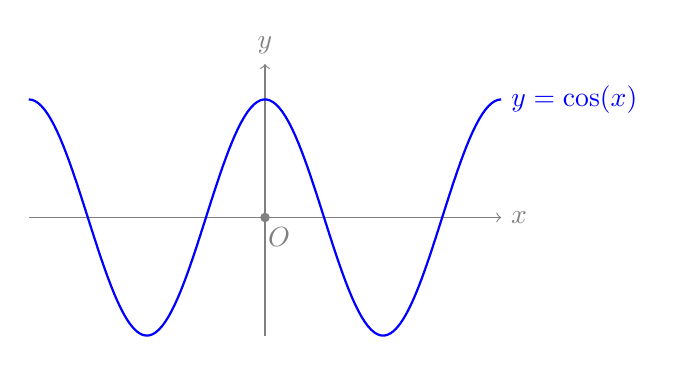
\begin{tikzpicture}[scale=1.5]
% Draw the x and y axis, label the axes and the origin
\draw[gray, ->] (-2,0) -- (2,0) node[right]{$x$} node[pos=0.53, below]{$O$};
\draw[gray, ->] (0,-1) -- (0,1.3) node[above]{$y$};
\draw[fill,gray] (0,0) circle [radius=1pt];
% Plot the curve
\draw[blue, thick] [domain=-2:2, samples=150] plot (\x, {cos(pi*\x r)}) node[right]{$y = \cos(x)$};
% Note: the r in the argument of the cosine signifies that we enter \x in radians↪
\end{tikzpicture}

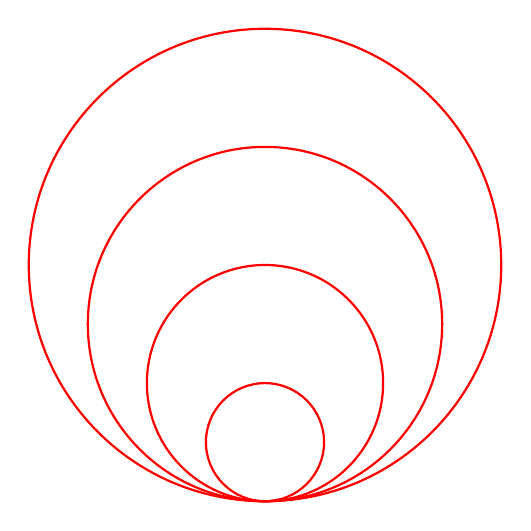
\begin{tikzpicture}[scale=0.75]
\foreach \x in {0,1,2,3}
\draw[red,thick] (0,\x) circle [radius=\x+1];
\end{tikzpicture}

\end{document}